\documentclass[11pt,a4paper]{article}
\usepackage[margin=2.5cm]{geometry}
\usepackage{graphicx}
\title{Labwork 7: Grayscale Stretch}
\author{Duong Tan Binh \\ Student ID: 2540007}
\date{}
\begin{document}
\maketitle
\section{Method}
I make a low-contrast input from the Lab 3 RGB image by dividing each
channel by 2 and adding 50. The GPU first converts it to grayscale.
Each block then finds its minimum and maximum using shared-memory reduction.
I use the last reduction loop from the slide: the stride starts at half
of the block and is divided by 2 at each step.
I repeat the reduction on the block results until only one minimum
and one maximum remain. Threads outside the image use 255 for minimum
and 0 for maximum, so they do not change the result.

The last kernel calculates \texttt{(gray - min) * 255 // (max - min)}.
For a constant image, I write 0 to avoid division by zero.

\section{Results}
I test three 2D block sizes. I compile the kernels before timing.
Times include the grayscale conversion, all reduction passes and their
allocations, stretch, and data transfers. Each configuration is measured once.
\begin{verbatim}
Block size: (8, 8)
Min: 50 Max: 177
Total time: 3.853 ms
Block size: (16, 16)
Min: 50 Max: 177
Total time: 2.121 ms
Block size: (32, 32)
Min: 50 Max: 177
Total time: 1.678 ms
\end{verbatim}
The input grayscale range is 50 to 177; the output range is 0 to 255.
All three configurations give the same result. The 32 by 32 block
has the lowest time in this run.

\begin{center}
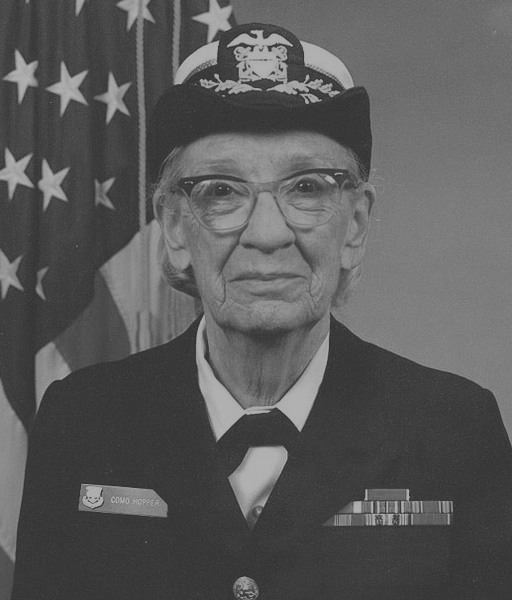
\includegraphics[width=0.32\textwidth]{gray.png}
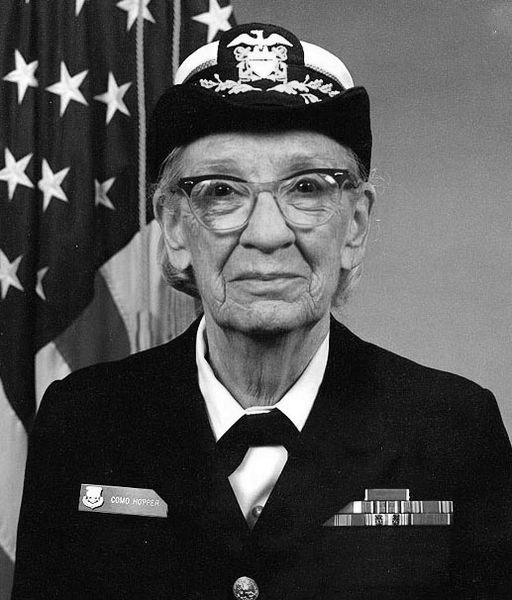
\includegraphics[width=0.32\textwidth]{stretched.png}
\end{center}
Grayscale input and stretched result.

\end{document}
